\documentclass[a4paper,11pt]{article}
\usepackage{amsmath,amsthm,amsfonts,amssymb,amscd,amstext,vmargin,graphics,graphicx,tabularx,multicol} 
\usepackage[francais]{babel}
\usepackage[utf8]{inputenc}  
\usepackage[T1]{fontenc} 
\usepackage{pstricks-add,tikz,tkz-tab,variations}
\usepackage[autolanguage,np]{numprint} 
\usepackage{xlop}


\setmarginsrb{1.5cm}{0.5cm}{1cm}{0.5cm}{0cm}{0cm}{0cm}{0cm} %Gauche, haut, droite, haut
\newcounter{numexo}
\newcommand{\exo}[1]{\stepcounter{numexo}\noindent{\bf Exercice~\thenumexo} : \marginpar{\hfill /#1}}
\reversemarginpar


\newcounter{enumtabi}
\newcounter{enumtaba}
\newcommand{\q}{\stepcounter{enumtabi} \theenumtabi.  }
\newcommand{\qa}{\stepcounter{enumtaba} (\alph{enumtaba}) }
\newcommand{\initq}{\setcounter{enumtabi}{0}}
\newcommand{\initqa}{\setcounter{enumtaba}{0}}

\newcommand{\be}{\begin{enumerate}}
\newcommand{\ee}{\end{enumerate}}
\newcommand{\bi}{\begin{itemize}}
\newcommand{\ei}{\end{itemize}}
\newcommand{\bp}{\begin{pspicture*}}
\newcommand{\ep}{\end{pspicture*}}
\newcommand{\bt}{\begin{tabular}}
\newcommand{\et}{\end{tabular}}
\renewcommand{\tabularxcolumn}[1]{>{\centering}m{#1}} %(colonne m{} centrée, au lieu de p par défault) 
\newcommand{\tnl}{\tabularnewline}

\newcommand{\bmul}[1]{\begin{multicols}{#1}}
\newcommand{\emul}{\end{multicols}}

\newcommand{\trait}{\noindent \rule{\linewidth}{0.2mm}}
\newcommand{\hs}[1]{\hspace{#1}}
\newcommand{\vs}[1]{\vspace{#1}}

\newcommand{\N}{\mathbb{N}}
\newcommand{\Z}{\mathbb{Z}}
\newcommand{\R}{\mathbb{R}}
\newcommand{\C}{\mathbb{C}}
\newcommand{\Dcal}{\mathcal{D}}
\newcommand{\Ccal}{\mathcal{C}}
\newcommand{\mc}{\mathcal}

\newcommand{\vect}[1]{\overrightarrow{#1}}
\newcommand{\ds}{\displaystyle}
\newcommand{\eq}{\quad \Leftrightarrow \quad}
\newcommand{\vecti}{\vec{\imath}}
\newcommand{\vectj}{\vec{\jmath}}
\newcommand{\Oij}{(O;\vec{\imath}, \vec{\jmath})}
\newcommand{\OIJ}{(O;I,J)}


\newcommand{\reponse}[1][1]{%
\multido{}{#1}{\makebox[\linewidth]{\rule[0pt]{0pt}{20pt}\dotfill}
}}

\newcommand{\titre}[5] 
% #1: titre #2: haut gauche #3: bas gauche #4: haut droite #5: bas droite
{
\noindent #2 \hfill #4 \\
#3 \hfill #5

\vspace{-1.6cm}

\begin{center}\rule{6cm}{0.5mm}\end{center}
\vspace{0.2cm}
\begin{center}{\large{\textbf{#1}}}\end{center}
\begin{center}\rule{6cm}{0.5mm}\end{center}
}



\begin{document}
\pagestyle{empty}
\titre{Interrogation sur les cercles et les triangles }{Nom :}{Prénom :}{Classe}{Date}


\vspace*{0.4cm}
\begin{flushleft}
\begin{tabular}{|m{9.5cm}|m{1.25cm}|m{1.25cm}|m{1.25cm}|m{1.25cm}|m{1.25cm}|}
\hline 
\textbf{Compétences} & \begin{center}
\textbf{N.E.}
\end{center} & \begin{center}
\textbf{M.I.}
\end{center} & \begin{center}
\textbf{M.F.}
\end{center}  & \begin{center}
\textbf{M.S.}
\end{center} & \begin{center}
\textbf{T.B.M.}
\end{center} \\ 
\hline 
Je dois connaître et savoir utiliser associé au cercle & & &  & &\\
\hline
Je dois savoir construire un triangle en connaissant les longueurs de ses côtés & & &  & & \\ 
\hline



\end{tabular}  
\end{flushleft}

\textit{N.E = Non évalué ; M.I. = Maîtrise insuffisante ; M.F. = Maîtrise fragile ; M.S. = Maîtrise satisfaisante ; T.B.M. = Très bonne maîtrise}\\

\vspace*{0.4cm}

\exo{1} Compléter les phrases suivantes à l'aide des mots vus en cours :

\bmul{2}

Le point O est . . . . . . . . . . . . . . . . . . . . . . du cercle.\\

$[AB]$ est . . . . . . . . . . . . . . . . . . . . . . du cercle.\\

Le point O est . . . . . . . . . . . . . . . .  du segment $[AM]$.\\

 $[AM]$ est . . . . . . . . . . . . . . . . . . . . . . du cercle.\\

\columnbreak


\begin{flushright}
\includegraphics[scale=0.75]{exointerrocercle3.eps} 
\end{flushright}



\emul


\exo{2} Sur la figure ci-dessous, tracer : \\
- 	le cercle de centre A et de rayon 2 cm ;\\
-	le cercle de centre K passant par B ;\\
-	le cercle de centre L et de diamètre 4 cm ;\\
-	le cercle de diamètre [NT].

\includegraphics[scale=0.85]{exointerrocercle4.eps} 


\newpage

\vspace*{0.5cm}

\exo{5} Tracer les 3 triangles suivants en vraie grandeur en respectant les dimensions données. Penser au codage des figures.\\

\q Tracer un triangle ABC tel que AB = 6 cm; AC = 5 cm et BC = 4 cm.\\

\vspace*{7cm}


\q Trace un triangle EFG isocèle en G tel que EG = 4,5 cm et EF = 7,2 cm.\\

\vspace*{8cm}

\q Trace un triangle RST rectangle en R tel que RT = 3,8 cm et ST = 6,5 cm\\

\vspace*{5cm}

\newpage

\vspace*{0.5cm}

\exo{2} Tracer en vraie grandeur la figure ci-dessous en respectant les longueurs données :

\begin{center}
\includegraphics[scale=0.5]{exointerrocercle1.eps} 
\end{center}

\vspace*{9cm}

\exo{}BONUS

\bmul{2}

\vspace*{0.4cm}
Combien y a-t-il de triangles sur l'image ci-contre? \\
\reponse[2]\\

\vspace*{0.7cm}

\columnbreak



\includegraphics[scale=0.6]{exointerrocercle2.eps} 

\emul


\end{document}
